\documentclass{standalone}

\usepackage{tikz}
\usetikzlibrary{arrows}

\begin{document}

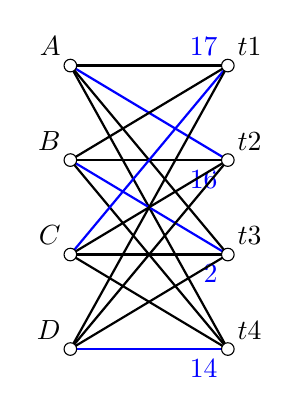
\begin{tikzpicture}[x=0.4cm,y=0.4cm]  %[scale=0.5]
\tikz
  % def workers
  \coordinate (A) at (0,10);
  \coordinate (B) at (0,7);
  \coordinate (C) at (0,4);
  \coordinate (D) at (0,1);
  % def work
  \coordinate (t1) at (5,10);
  \coordinate (t2) at (5,7);
  \coordinate (t3) at (5,4);
  \coordinate (t4) at (5,1);
  
  %stile frecce
  \tikzset{arc/.style={-, black, fill=none, thick, >=stealth, text=black}} %%->


  %frecce
  \draw[arc, color = black] (A) -- (t1) ;
  \draw[arc, color = blue] (A) -- (t2) node[below left] {16};
  \draw[arc, color = black] (A) -- (t3);
  \draw[arc, color = black] (A) -- (t4);
  
  \draw[arc, color = black] (B) -- (t1);
  \draw[arc, color = black] (B) -- (t2);
  \draw[arc, color = blue] (B) -- (t3) node[below left] {2};
  \draw[arc, color = black] (B) -- (t4);
  
  \draw[arc, color = blue] (C) -- (t1) node[above left] {17};;
  \draw[arc, color = black] (C) -- (t2);
  \draw[arc, color = black] (C) -- (t3);
  \draw[arc, color = black] (C) -- (t4);
  
  \draw[arc, color = black] (D) -- (t1);
  \draw[arc, color = black] (D) -- (t2);
  \draw[arc, color = black] (D) -- (t3);
  \draw[arc, color = blue] (D) -- (t4) node[below left] {14};;
  
  % pallini
  \filldraw[fill=white] (A) circle(.2);
  \filldraw[fill=white] (B) circle(.2);
  \filldraw[fill=white] (C) circle(.2);
  \filldraw[fill=white] (D) circle(.2);
  \filldraw[fill=white] (t1) circle(.2);
  \filldraw[fill=white] (t2) circle(.2);
  \filldraw[fill=white] (t3) circle(.2);
  \filldraw[fill=white] (t4) circle(.2);

  %etichette
  \node[above left] at (A) {$A$};
  \node[above left] at (B) {$B$};
  \node[above left] at (C) {$C$};
  \node[above left] at (D) {$D$};
  
  \node[above right] at (t1) {$t1$};
  \node[above right] at (t2) {$t2$};
  \node[above right] at (t3) {$t3$};
  \node[above right] at (t4) {$t4$};
  

\end{tikzpicture}

\end{document}